\documentclass{article}
\usepackage[backend = biber, bibstyle = apa, citestyle = apa, style = apa, sorting = none, sortcites = true, block = none]{biblatex}
\usepackage[utf8]{inputenc}
\usepackage{csquotes}
\usepackage[spanish]{babel}
\usepackage[]{amsthm}
\usepackage{amsmath}
\usepackage[]{amssymb}
\usepackage{graphicx}
\usepackage{wrapfig}
\usepackage[letterpaper, margin=1.5in]{geometry}
\usepackage[hidelinks]{hyperref}
\decimalpoint

\graphicspath{img/}
\addbibresource{references.bib}

\begin{document}
    \begin{titlepage}
        \begin{center}
            \begin{figure}
                \centering
                
\includegraphics[scale=0.13]{logo_itesm.png}\\ % Logo de la institución
            \end{figure}
        \vspace{5cm}
        \LARGE{Instituto Tecnológico y de Estudios Superiores de Monterrey}\\
        \fontsize{12}{14}\selectfont
        \vspace{1cm}
        \textbf{Reporte final del reto}\\ % Nombre de la tarea
        \vspace{0.7cm}
        Juan Pablo Echeagaray González\\ % Nombre de autor 1
        \vspace{0.2cm}
        A00830646\\ % Matrícula autor 1
        \vspace{0.7cm}
        Análisis de Ciencias de datos\\ % Materia
        \vspace{0.2cm}
        TC2004B.100\\ % Clave de la materia
        \vspace{0.2cm}
        Daniel Otero Fadul\\ % Nombre del profesor
        \vspace{0.7cm}
        19 de marzo del 2022\\ % Fecha de entrega
        \end{center}
    \end{titlepage}

    \section{Introducción}
        La organización CENGAGE es una compañía que otorga recursos educacionales físicos y digitales a instituciones de educación superior como bachillerato y universidad. CENGAGE quiere conocer su posible rendimiento en el futuro cuando la pandemia concluya. Dado esta inquietud, la compañía otorgó sus datos históricos durante el periodo de tiempo de los últimos 2 años para realizar un pronóstico de su desempeño en los meses por venir.

    \section{Objetivos}
        \subsection{Objetivo general}
        Modelar los datos de ventas para predecir con mayor seguridad las ganancias generadas de una operación.

        \subsection{Objetivos específicos}
            \begin{itemize}
                \item Leer y limpiar la base de datos de las ventas realizadas entre el año 2020 y 2021, esto incluye la eliminación de columnas sin datos y entradas atípicas.
                \item Procesar cada variable en la base de datos para su descripción.
                \item Modificar variables para mejorar la interpretación de las mismas. 
                \item Analizar las correlaciones entre variables para identificar relaciones entre ellas.
                \item Visualizar la información para la elaboración de modelos predictivos y evaluarlos según diferentes métricas de desempeño. 
            \end{itemize}

    \section{Justificación}
        Se realizó este análisis de la base de datos brindada por CENGAGE con el fin de predecir los futuros ingresos de la compañía y el ingreso que genera cada operación, ya que el tener una visión a futuro puede ser bastante útil, puesto que el tener un estimado de ventas en los periodos por venir ayuda a visualizar los posibles nuevos gastos que se pueden permitir.

        Al predecir los ingresos futuros también incluyen otras ventajas, como lo es el visualizar y analizar cuales son las principales fuentes de ingresos de la compañía, por lo que en ese espacio pueden invertir más en ello, así como ir eliminando o reduciendo recursos a ciertos productos que no aporten una cantidad significante.
        
        Así mismo, con la llegada de la pandemia de COVID-19 afectó directamente a la compañía en sus ventas. Sin embargo, este suceso se ve pronosticado a acabarse de manera próxima, lo cual se verá reflejado en el ingreso de CENGAGE. Por eso mismo, se buscó realizar una predicción de las ganancias de una operación a partir de los datos proporcionados del año 2020 hasta el 2021.

    \section{Metodología}

        Para realizar el procesamiento de datos, análisis exploratorio y predictivo hemos optado por utilizar el lenguaje de programación Python con algunas de las librerías más usadas por la comunidad, en específico:

        \begin{itemize}
            \item \emph{Numpy} \parencite{numpy}, \emph{Scipy} \parencite{2020SciPy-NMeth}: Operaciones matemáticas
            \item \emph{Pandas} \parencite{reback2020pandas}: Lectura y manipulación de datos
            \item \emph{Seaborn} \parencite{seaborn}, \emph{Matplotlib} \parencite{matplotlib}: Visualización de datos
            \item \emph{Scikit-learn} \parencite{scikit-learn}: Modelos predictivos
        \end{itemize}

        \subsection{Procesamiento de datos}

        Para iniciar el proceso de análisis de la base de datos se importaron los datos y se analizó su estructura. La base de datos otorgada cuenta con 24,862 entradas en donde se capturaron un total de 24 variables como se puede observar en la siguiente imagen:

        \begin{figure}[h]
            \centering
            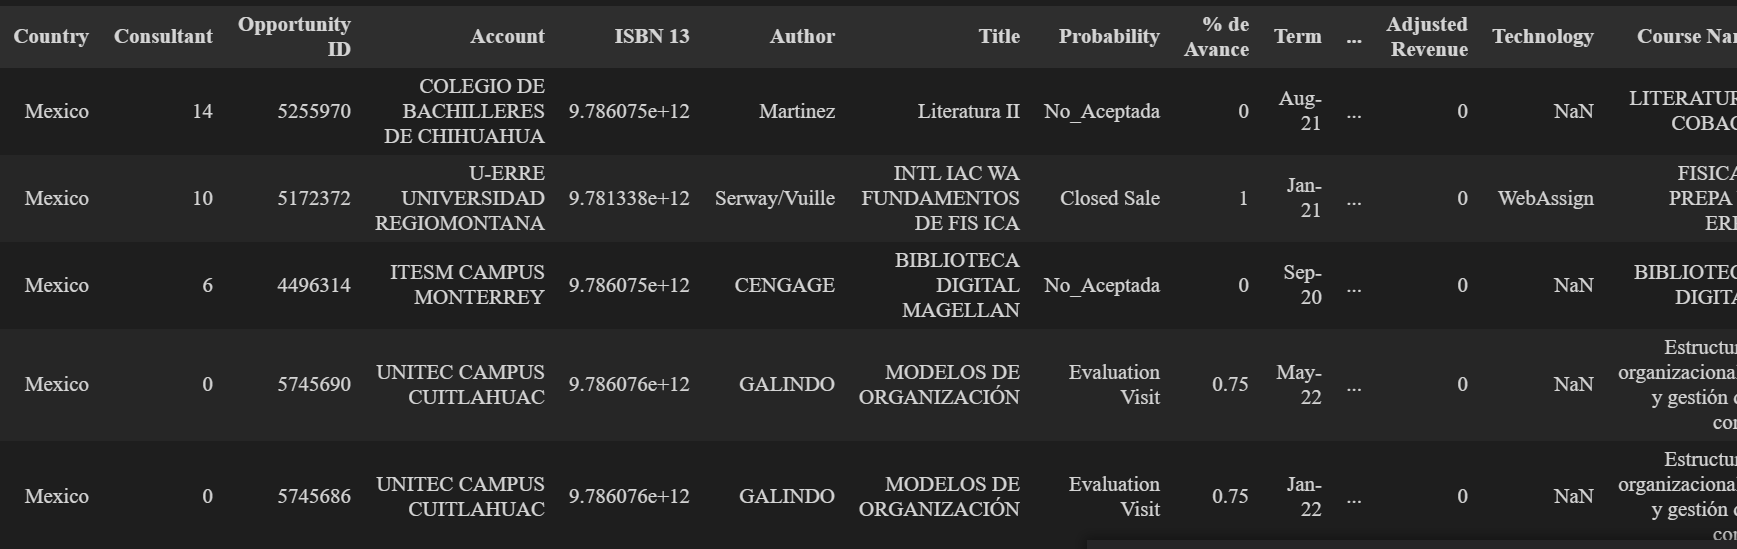
\includegraphics[width=\columnwidth]{tablaSinLimpieza.png}
            \caption{Encabezado de la base de datos sin modificación}
            \label{fig:table}
        \end{figure}


        Sin embargo, las 24 variables enumeradas en la tabla no se encuentran en todas las entradas. La Figura \ref{fig:propValNul} muestra la proporción de valores nulos por columna o variable capturada entre todos los registros. Se definió un valor límite de esta proporción de 0.7, mostrando 4 de las 24 variables que superan esta proporción, por lo que las columnas 'New Course Takeaway Units' , '$\#$ of Courses', 'Unlimited Flag' e 'Implementation Id' fueron removidas para la limpieza de datos, pues no figuraban para el análisis.
        \newpage
        \begin{figure}[h!]
            \centering
            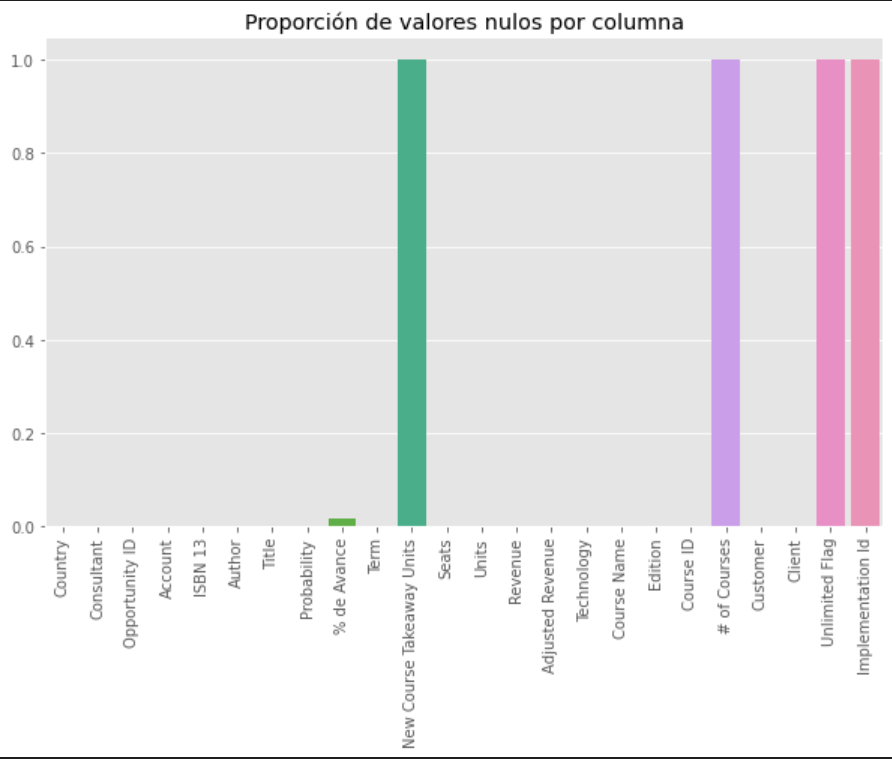
\includegraphics[width=\columnwidth]{proporcionNulos.png}
            \caption{Proporción de valores nulos por columna}
            \label{fig:propValNul}
        \end{figure}

        Dentro de la base de datos se ha eliminado las variables no tan presentes en la mayoría de las entradas, por lo que se puede empezar a visualizar aquellas variables que sí son abundantes por cada entrada. Un ejemplo de una visualización que se realizó es la relación entre ingresos con el tiempo, esto se puede apreciar en la Figura \ref{fig:revenue} y en la Figura \ref{fig:revenueCons} se muestra el ingreso generado por cada consultor de la empresa.
        También podemos observar en la Figura \ref{fig:revenue} los picos del ingreso generado en los meses de agosto y enero, dando a entender que se genera mayores ingresos durante los periodos de inicio de clases, tanto para el periodo de verano como de invierno.

        \newpage
        \begin{figure}[h]
            \centering
            \includegraphics[width=\columnwidth]{output.png}
            \caption{Ingreso por Consultor}
            \label{fig:revenueCons}
        \end{figure}


        \begin{figure}[h]
            \centering
            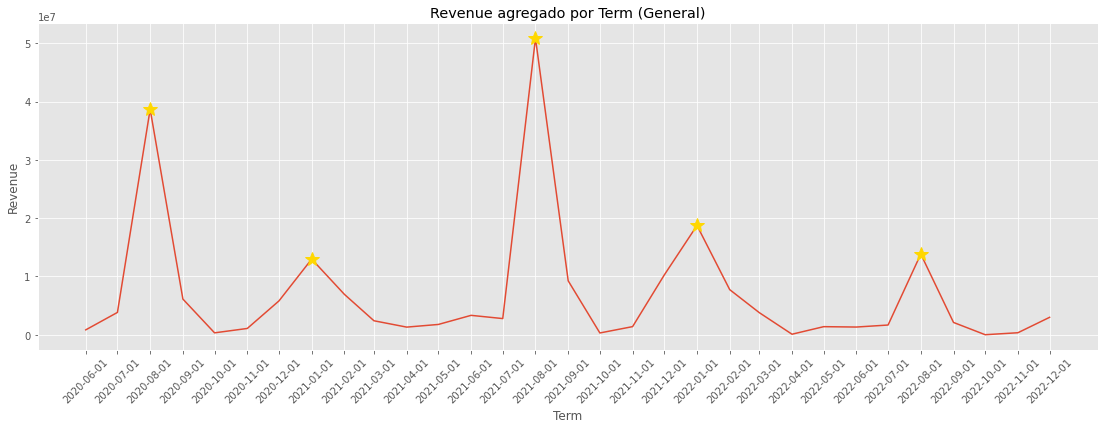
\includegraphics[width = \columnwidth]{revenue.png}
            \caption{Ingresos de CENGAGE}
            \label{fig:revenue}
        \end{figure}

        Por otro lado también se eliminó la variable 'Adjusted Revenue' debido a que se encontraba con valores nulos y dado esto era necesario dejarla fuera de un análisis predictivo o de clasificación.


        
        \vspace{3 mm}
        
        Con el uso de la variable 'Probability' se le asignó una posible probabilidad a cada una de las diferentes clasificaciones, con el fin de poder obtener un valor numérico de estas y medir el peso que tienen a la hora de realizar una venta. Esto nos ayudará más adelante, al momento de entrar al análisis exploratorio.
        
        \subsection{Análisis exploratorio}
        
        El próximo paso para el análisis de los datos es identificar qué pares de variables numéricas tienen una correlación lo suficientemente alta para ser evaluadas y consideradas para el modelo de predicción. La matriz de correlación mostrada en la Figura \ref{fig:tablaCor} explica esta relación, entre más alto sea el valor absoluto, más correlación existirán entre ambas variables. Por ejemplo, la variable Units y la variable Revenue tienen una correlación de +0.567, que significa que hay una buena relación ascendente entre la cantidad de unidades vendidas en un pedido y el monto de ingreso por el pedido.

        \begin{figure}[h!]
            \centering
            \includegraphics[width = \columnwidth]{new_cor_matrix.png}
            \caption{Matriz de Correlación de los Datos}
            \label{fig:tablaCor}
        \end{figure}
        Así mismo, la matriz utiliza solamente variables numéricas, ya que para la hora de realizarla las variables categóricas no tomaron un papel en esto, generando así una matriz más limpia y fácil de entender. 

        \newpage

        \begin{figure}[h!]
            \centering
            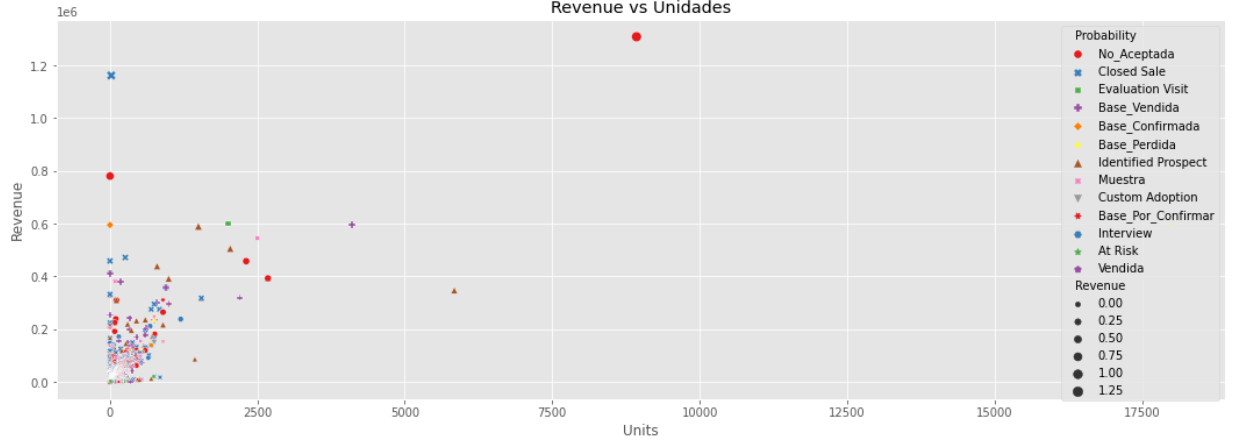
\includegraphics[width = \columnwidth]{Revenue vs Unit.PNG}
            \caption{Ingresos por Unidad}
            \label{fig:revUnit}
        \end{figure}

        En la Figura \ref{fig:revUnit} se utilizó la información de múltiples variables para poder generar la visualización presentada, como lo son las variables 'Units', 'Revenue', 'Probability' y 'Set1'. En esta figura se presenta el ingreso que cada una de las clasificaciones proporciona dependiendo de la cantidad de unidades vendidas, así como mostrar también la probabilidad de que estas sucedan.

        \vspace{3mm}

        \begin{figure}[h!]
            \centering
            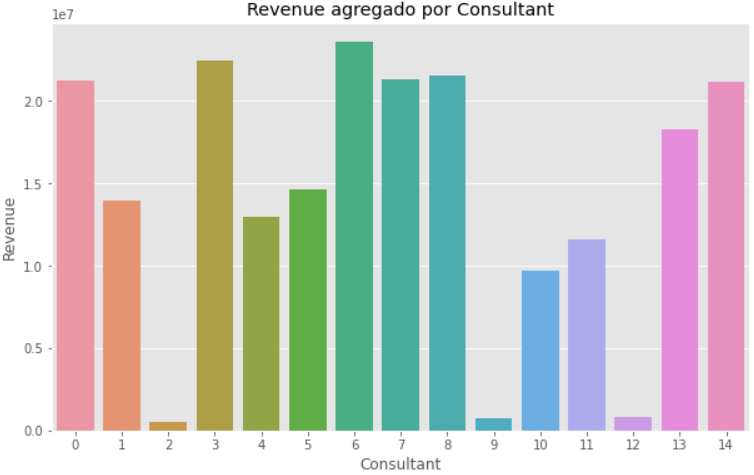
\includegraphics[width = \columnwidth]{Revenue por Consultor.PNG}
            \caption{Ingresos por Consultor}
            \label{fig:revConsultor}
        \end{figure}

        Posteriormente se procedió a generar una gráfica que se concentra de manera principal en mostrar la contribución de cada uno de los consultores de CENGAGE a lo largo del lapso presentado por la base de datos. Esto con ayuda de 'groupby', lo cual permite separar los valores del Revenue por cada uno de los diferentes consultores que se nos brindan en la base de datos. Obteniendo como resultado valores bastante altos para algunos de los consultores, mientras que otros tienen ingresos bastante bajos.

        \begin{figure}[h!]
            \centering
            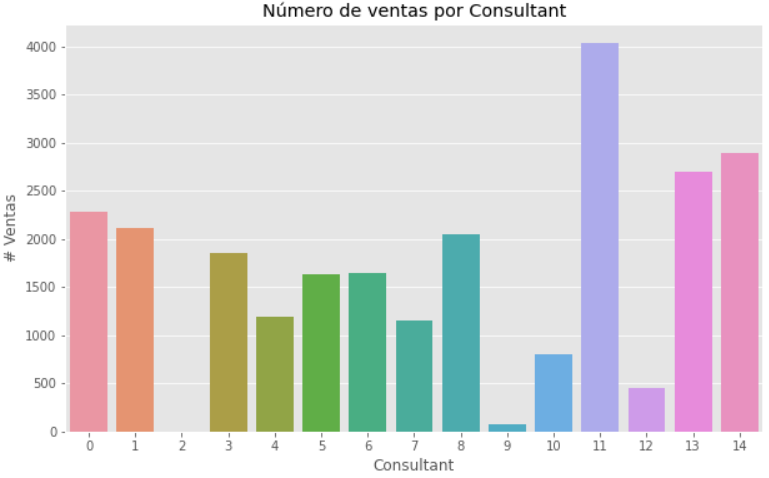
\includegraphics[width = \columnwidth]{Ventas por Consultor.PNG}
            \caption{Ventas por Consultor}
            \label{fig:ventConsultor}
        \end{figure}

        Consecutivamente se realizó una gráfica que relaciona el número de ventas realizadas con cada uno de los consultores, esto puede ser visualizado en la Figura \ref{fig:ventConsultor}. Esto nos permite percatarnos de que hay algunos consultores que generan más ventas que otros, siendo el consultor número 11 el que más destaca, teniendo alrededor de 4000 ventas realizadas en el lapso de tiempo utilizado, así como poco más de 1000 ventas por arriba del segundo consultor que más ventas realizó.


        \begin{figure}[h!]
            \centering
            \includegraphics[width = \columnwidth]{Revenue por título.PNG}
            \caption{Ingresos por Título}
            \label{fig:revTítulo}
        \end{figure}

        Una vez ya analizados los consultores, se continuó a analizar los títulos más vendidos y nuevamente se volvió a hacer uso de 'groupby' para poder separar los datos, tomando solo los 15 más altos con el fin de hacer más amena la visualización de los demás títulos, así como tomar en cuenta los que más aportan a CENGAGE. Al obtenerse los títulos se acomodaron de tal forma que los que tuvieran un ingreso más alto estuvieran del lado izquierdo, mientras que los de ingresos más bajos al lado derecho. Esto mostró que el título que más ingresos aportó durante el periodo este periodo de tiempo fue la Biblioteca digital magellan.

        \begin{figure}[h!]
            \centering
            \includegraphics[width = \columnwidth]{Ventas por título.PNG}
            \caption{Ventas por Título}
            \label{fig:ventTítulo}
        \end{figure}

        En la Figura \ref{fig:ventTítulo} se muestra el número de ventas por cada uno de los títulos que se tienen, nuevamente, tomando solo los primeros 15, puesto son los más significativos. En esta gráfica se muestra una diferencia bastante pronunciada entre el título con mayor número de ventas y el segundo lugar. El título que más ventas tuvo fue el de Intl epin ewa generic homework w/ebk, con un número superior a 50,000 unidades vendidas; mientras que el segundo con más ventas tuvo poco más de 20,000 unidades; viéndose clara la diferencia entre estos dos títulos.

        \begin{figure}[h!]
            \centering
            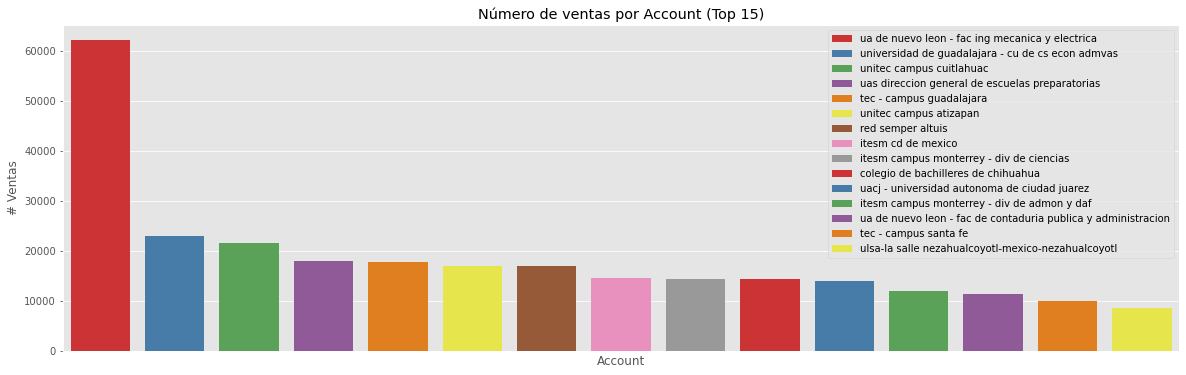
\includegraphics[width = \columnwidth]{VentasVSAccount.png}
            \caption{Los mejores clientes}
            \label{fig:ventClientes}
        \end{figure}

        Podemos observar en la Figura \ref{fig:ventClientes} los 15 mejores clientes que tiene la compañía respecto al número de ventas. Teniendo con una gran diferencia al número uno a la Universidad Autónoma de Nuevo León - Fac. ing. mecánica y eléctrica con una venta de más de 60,000.

        \newpage

        \subsection{Modelos predictivos}

        Después de haber completado el análisis exploratorio se prosiguió a realizar los modelos de "machine learning". Antes de pasar como tal a esa parte, cabe mencionar que para la selección de variables se hizo uso de lo que se conoce como One Hot Encoding, el cual a grandes rasgos consiste en generar una nueva columna por cada uno de los valores distintos que existan en dicha categoría. Esto se realizó de manera principal utilizando el paquete 'sklearn' y con esto se agregaron 20 nuevas variables, siendo procedentes de las variables 'Technology' y 'Country'.

        \vspace{4mm}

        Al haber utilizado el One Hot Encoding se generaron una gran cantidad de variables nuevas, las cuales pueden ocasionar que los modelos no se acoplen correctamente a datos nuevos a la hora de modelarlos si todas las variables son utilizadas.

        \vspace{4mm}

        Posteriormente se estandarizaron los datos, con el fin de que estos tuvieran el mismo rango que los demás, puesto que si no estuvieran de esta manera al momento de operar con ellas pueden existir inconsistencias y algunos problemas con los resultados debido a que no todas las variables trabajan entre los mismos valores. Para lograr esto se hizo uso de las funciones \emph{StandardScaler} y de \emph{fit\_transform}, las cuales pertenecen a \emph{sklearn} \parencite{scikit-learn}. Ahora que ya se encuentran estandarizados los datos, se pueden realizar conjuntos, algunos con los datos estandarizados y otros aún sin estandarizar. Esto último más que nada para realizar la comparación de los resultados de los distintos modelos a la hora de haber utilizado los valores de manera estandarizada y de no usarlos. Dichos conjuntos fueron necesarios para hacer tanto el grupo de entrenamiento como el de prueba.

    \section{Resultados y conclusiones}
        Después de las pruebas iniciales vemos que los modelos lineales no son capaces de capturar las relaciones que hay entre las variables numéricas de la base de datos y el Revenue logrado; el único regresor que tuvo un desempeño prometedor fue el árbol de decisión. De ahora en adelante nos enfocaremos en optimizar este método, encontrando los parámetros que maximicen su poder predictivo.

        Reducción de dimensionalidad: se comparan las medidas de desempeño para nuestros modelos iniciales usando el dataframe que contiene las 20 variables nuevas. Este conjunto de datos fue a su vez usado estandarizado y sin estandarizar. Ahora que ya sabemos que de entre todos, los árboles de decisión regresores que usan datos estandarizados son los que tienen un mejor desempeño, podemos enfocarnos en verificar si es que podemos reducir el número de variables que los modelos utilicen.
        
        Vemos que la mayoría de las variables no tienen mucha importancia para el modelo en general. Podemos descartar la mayoría y solamente quedarnos con unas cuantas. Como equipo proponemos quedarnos con las mejores 5:
        
        \begin{enumerate}
            \item Units
            \item Seats
            \item Country$_$Mexico
            \item Consultant
            \item Edition 
        \end{enumerate}
        
        Los valores de importancia representados en la Figura 12 son una representación directa del valor predictivo que tienen para el árbol regresor.
        
        Los distintos modelos realizados para predecir el comportamiento de las ventas de la compañía otorgaron diferentes resultados en cuanto a su desempeño: unos calificaban bien en cuanto a su poder predictivo, otros tuvieron menor error entre el valor real y el valor del modelo, y otros se ajustaban mejor a la gráfica de ingresos contra el tiempo. Sin embargo, hubo un modelo que resaltaba más que los demás: este modelo es el Árbol Regresor Estandarizado.
        
        El modelo Árbol Regresor o Árbol de Decisión Estandarizado se enfoca en analizar los datos de entrada a través de ciertas condiciones que estas variables cumplan: ¿Las unidades pedidas sobrepasan de cierto valor? ¿Qué consultor está manejando el pedido? ¿La edición que se dará al posible cliente es reciente o antigua? Estas clases de preguntas ayudan al modelo a predecir con cierto nivel de certeza el ingreso que se va generar por dicho pedido.
        
        Sin embargo, ciertas variables en el pedido otorgarán más información a la predicción que otras, y es por ello que la Figura \ref{fig:importance} muestra el nivel de importancia de cada una de esta variables para la predicción de ingresos.
        
        La Figura \ref{fig:model} muestra una comparativa de los ingresos reales de CENGAGE y aquellos predichos por nuestro modelo.
        Después de realizar la validación cruzada y el GridSearch, encontramos que en promedio un árbol de decisión regresor tendrá un puntaje de 58.16 \% , y que la mejor variante de árbol de decisión regresor es aquella que tiene una máxima profundidad de 19, su coeficiente de determinación es de 75.82\%
        
        Con este modelo CENGAGE podría atribuir el 75.82\% de sus ganancias generadas a las predicciones del modelo.
        
        \begin{figure}[h]
            \centering
            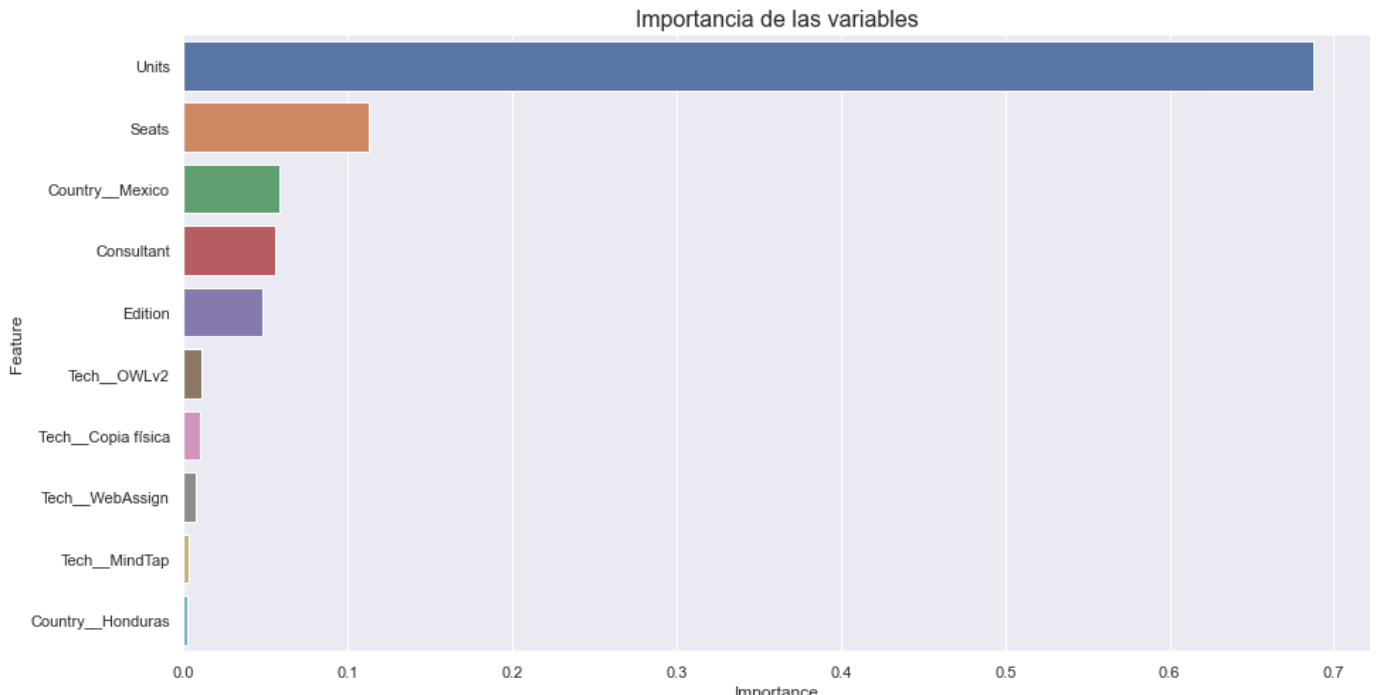
\includegraphics[width=\columnwidth]{importance.png}
            \caption{Nivel de Importancia por Variable en el Modelo Árbol Regresor}
            \label{fig:importance}
        \end{figure}
        
        \begin{figure}
            \centering
            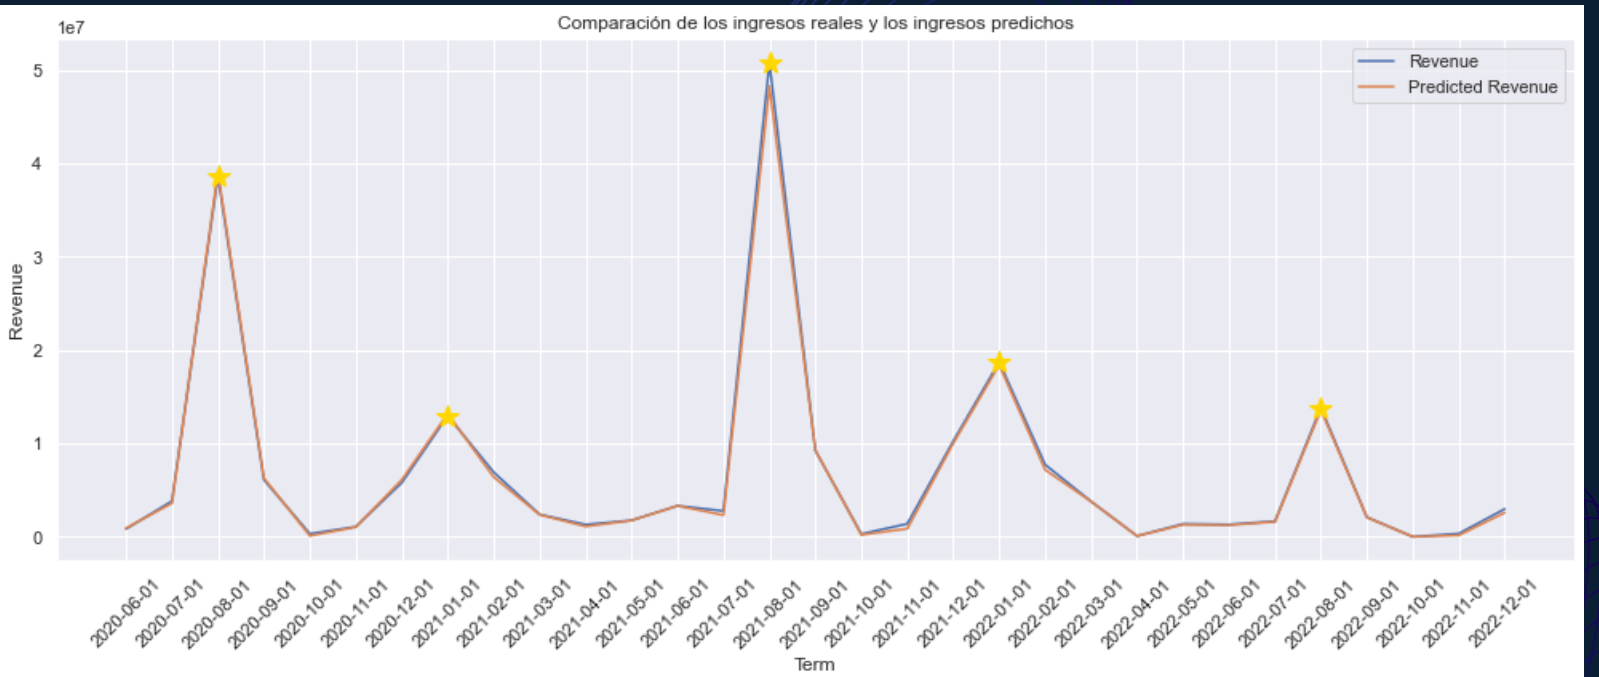
\includegraphics[width = \columnwidth]{model.png}
            \caption{Gráfica de los Ingresos y el Modelo Árbol Regresor}
            \label{fig:model}
        \end{figure}

    \section{Conclusiones}
        Después de realizar predicciones con siete modelos distintos y aplicar el proceso de validación cruzada, nos basamos en sus métricas para decidir cuál era el más acertado. Al observar el coeficiente de determinación $R^{2}$ de cinco de los modelos, nos dimos cuenta que eran cercanos a cero, por lo que de inmediato los descartamos en el proceso. De hecho, al observar el Error Cuadrático Medio (MSE) de estos, eran muy elevados a comparación de los modelos que no descartamos.
        
        Los únicos modelos factibles eran el de Árbol de Decisión Regresor o el de Árbol de Decisión Regresor Estandarizado, pero después de nuestro proceso de investigación hemos encontrado que un Árbol de Decisión Regresor con profundidad máxima de 19 tiene la mejor capacidad de predecir el Revenue generado por una operación dada. El modelo que encontramos tiene un coeficiente de determinación $R^{2}$ de 0.7582, y MSE (Error Cuadrático Medio) de 0.403 el cual, como vimos en la Figura 13, se adaptaba muy bien a los ingresos de CENGAGE reales. Es posible darse cuenta de esto en las pequeñas diferencias que tenían las líneas del modelo y las reales, imperceptibles a simple vista.
        
        Como recordatorio, tiene que hacerse una transformación de la predicción generada por el modelo, actualmente los datos que regresa la predicción son valores logarítmicos, las ganancias predichas deben de ser exponenciadas para obtener las ganancias reales.

    \section{Contribuciones}
        \begin{itemize}
            \item \textbf{Juan Pablo Echeagaray González:} Implementación, pre-procesamiento, análisis y entrenamiento de modelos predictivos
            \item \textbf{Grace Aviance Silva Aróstegui:} Redacción del reporte y presentación
            \item \textbf{Emily Rebeca Méndez Cruz:} Visualizaciones, redacción del reporte y presentación
            \item \textbf{Eugenio Santisteban Zolezzi:} Pre-procesamiento de datos y redacción del reporte
            \item \textbf{Taurino López González:} Pre-procesamiento de datos y redacción del reporte
            \item \textbf{Ricardo de Jesús Balam Ek:} Resultados y  conclusiones en la redacción del reporte.
        \end{itemize}


    \clearpage
    \nocite{*}
    \printbibliography
\end{document}